%
% demodulation.tex -- Demodulation von QAM
%
% (c) 2020 Prof Dr Andreas Müller, Hochschule Rapperswil
%
\subsection{Demodulation
\label{subsection:demodulation}}
Die modulierten Komponenten $s(t)$ und $c(t)$ entstehen gemäss
\eqref{eqn:qam:modulation}
durch eine sehr rasche Drehung $D_{\omega t}\vec{v}(t)$
des Vektor $\vec{v}(t)$.
Da die Drehung durch eine Matrix beschrieben wird, können wir
sie auch wieder rückgängig machen, indem wir mit der inversen
Matrix
\[
D^{-1}_{\omega t} = D_{-\omega t}
=
\begin{pmatrix}
\phantom{-}\cos\omega t & \sin\omega t \\
         - \sin\omega t & \cos\omega t
\end{pmatrix}
\]
multiplizieren.
So finden wir
\[
D_{\omega t}^{-1}
\begin{pmatrix}s(t)\\c(t)\end{pmatrix}
=
D_{\omega t}^{-1}
D_{\omega t}^{\mathstrut}
\begin{pmatrix} I(t)\\Q(t)\end{pmatrix}
=
\begin{pmatrix}
I(t)\\
Q(t)
\end{pmatrix}.
\]
Es ist also klar, dass man aus $s(t)$ und $c(t)$ die ursprünglichen Signale
$I(t)$ und $Q(t)$ rekonstruieren kann.
Allerdings ist auch dies nicht wirklich eine Lösung des Problems.
Es ist immer noch notwendig, die beiden Funktionen $s(t)$ und $c(t)$
getrennt zu übertragen, um $I(t)$ und $Q(t)$ wiederzugewinnen.

\subsubsection{Demodulation mit Trigonometrie}
Wir suchen ein Verfahren, mit dem wir $I(t)$ und $Q(t)$ allein aus
$s(t)$ zurückgewinnen können.
Auch für dieses Problem suchen wir eine geometrische Lösung.
Wir gehen dazu von der Gleichung
\[
\vec{v}(t)
=
D_{-\omega t}\underbrace{D_{\omega t}
\vec{v}(t)}_{=\begin{pmatrix}s(t)\\c(t)\end{pmatrix}
\]
aus.
Die Tatsache, dass wir $c(t)$ nicht übertragen wollen, können wir dadurch
abbilden, dass wir in der Gleichung eine Projektionsmatrix $P$
verwenden, um die Komponeten $c(t)$ zu unterdrücken:
\[
P=\begin{pmatrix}1&0\\0&0\end{pmatrix}
\qquad\Rightarrow\qquad
P\begin{pmatrix}s(t)\\c(t)\end{pmatrix}
=
\begin{pmatrix}s(t)\\0\end{pmatrix}.
\]
Durch diese Änderung wird man natürlich nicht mehr $I(t)$ und $Q(t)$ 
zurückgewinnen können, stattdessen wird man modifizierte Funktionen
$\hat{I}(t)$ und $\hat{Q}(t)$ erhalten.
Das ganze Übertragung\-system könnte daher mit dem Matrizenprodukt
\[
\begin{pmatrix}
\hat{I}(t)\\
\hat{Q}(t)
\end{pmatrix}
=
D_{-\omega t} \begin{pmatrix}s(t)\\0\end{pmatrix}
=
D_{-\omega t} P D_{\omega t}\vec{v}(t)
\]
beschrieben werden.
Wegen
\[
D_{-\omega t}P
=
\begin{pmatrix}
\phantom{-}\cos\omega t & 0 \\
         - \sin\omega t & 0
\end{pmatrix}
\]
bedeutet dies
\begin{align*}
\hat{I}(t) &= \phantom{-}\cos\omega t s(t),\\
\hat{Q}(t) &= -\sin\omega t s(t).
\end{align*}
Wir bezeichnen den Vektor mit diesen Komponenten als
\[
\hat{v}(t) = \begin{pmatrix}\hat{I}(t)\\\hat{Q}(t)\end{pmatrix}.
\]
Der Vektor ist also das, was von der Rekonstruktion nach dem Wegfallen
der Komponente $c(t)$ noch übrig bleibt.

Wie unterscheiden sich $\hat{I}(t)$ und $\hat{Q}(t)$ von $I(t)$ und $Q(t)$?
Dazu berechnen wir
\begin{align*}
D_{-\omega t}PD_{\omega t}
&=
\begin{pmatrix}
\phantom{-}\cos\omega t & \sin\omega t \\
         - \sin\omega t & \cos\omega t
\end{pmatrix}
\begin{pmatrix} 1 & 0 \\ 0 & 0 \end{pmatrix}
\begin{pmatrix}
\cos\omega t &          - \sin\omega t \\
\sin\omega t & \phantom{-}\cos\omega t
\end{pmatrix}
\\
&=
\begin{pmatrix}
 \cos^2\omega t           & -\cos\omega t \sin\omega t \\
-\cos\omega t \sin\omega t&\sin^2\omega t
\end{pmatrix}
=
\frac12
\begin{pmatrix}
1+\cos 2\omega t &  -\sin 2\omega t \\
 -\sin 2\omega t & 1-\cos 2\omega t
\end{pmatrix}
\\
&=
\frac12 E + \frac12
\begin{pmatrix}
 \cos 2\omega t & -\sin 2\omega t \\
-\sin 2\omega t & -\cos 2\omega t
\end{pmatrix}.
\end{align*}
Im zweitletzten Schritt haben wir die Doppelwinkelformeln für
die trigonometrischen Funktionen verwendet.
Nach der Rekonstruktion bleiben also zwei Terme
\[
\hat{v}(t)
=
\frac12\vec{v}(t)
+
\frac12
\begin{pmatrix}
\phantom{-}\cos 2\omega t & -\sin 2\omega t \\
         - \sin 2\omega t & -\cos 2\omega t
\end{pmatrix}\vec{v}(t).
\]
Der erste Term ist bis auf den Faktor $\frac12$ der gesuchte
Vektor $\vec{v}(t)$.
Doch was ist der zweite Term?
Die Matrix kann man auch schreiben als
\begin{align*}
\begin{pmatrix}
\phantom{-}\cos2\omega t&-\sin2\omega t\\
         - \sin2\omega t&-\cos2\omega t
\end{pmatrix}
&=
\underbrace{
\begin{pmatrix}
1& 0\\
0&-1
\end{pmatrix}}_{\displaystyle = S}
\begin{pmatrix}
\cos2\omega t &          - \sin2\omega t \\
\sin2\omega t & \phantom{-}\cos2\omega t
\end{pmatrix}
=
\begin{pmatrix}
1& 0\\
0&-1
\end{pmatrix}
D_{2\omega t},
\end{align*}
bis auf die Spiegelungsmatrix $S$ handelt es sich also wieder um eine
Drehung, allerdings mit der doppelten Frequenz.
Beides zusammen kann kurz als
\begin{equation}
\hat{v}(t)
=
\frac12 \vec{v}(t)
+
\frac12 SD_{2\omega t}\vec{v}(t)
\label{eqn:qam:filter}
\end{equation}
geschrieben werden.

Die untersten zwei Graphen in Abbildung~\ref{figure:qam:sep} zeigen
die Komponenten $\hat{I}(t)$ und $\hat{Q}(t)$.
Es ist gut erkennbar, wie sie sich zusammensetzen aus $\frac12I(t)$ 
bzw.~$\frac12Q(t)$ überlagert mit einer Schwingung mit der doppelten
Frequenz des Trägers.

\subsubsection{Demodulation mit Matrixalgebra}
In der vorangegangenen Herleitung der Formel~\eqref{eqn:qam:filter}
haben wir ausgiebig von trigonometrischen Formeln Gebrauch gemacht.
Wir können die Formel aber auch auf eine viel geometrischere Art verstehen.
Dazu schreiben wir die Projektionsmatrix $P$ als eine Summe
\[
P
=
\begin{pmatrix}1&0\\0&0\end{pmatrix}
=
\begin{pmatrix}\frac12+\frac12&0\\0&\frac12-\frac12\end{pmatrix}
=
\frac12\begin{pmatrix}1&0\\0&1\end{pmatrix}
+
\frac12\begin{pmatrix}1&0\\0&-1\end{pmatrix}
=
\frac12E+\frac12S.
\]
Damit wird
\[
D_{-\omega t}PD_{\omega t}
=
\frac12D_{-\omega t}ED_{\omega t}
+
\frac12D_{-\omega t}SD_{\omega t}
=
\frac12E
+
\frac12D_{-\omega t}SD_{\omega t}.
\]
Wir wollen das Produkt $D_{-\omega t}S$ geometrisch verstehen und
modifizieren.
Die Matrix $S$ spiegelt Vektoren an der $I$-Achse, die Matrix $D_{-\omega t}$
dreht Vektoren um den Winkel $-\omega t$
(Abbildung~\ref{figure:qam:spiegelung}).
\begin{figure}
\centering
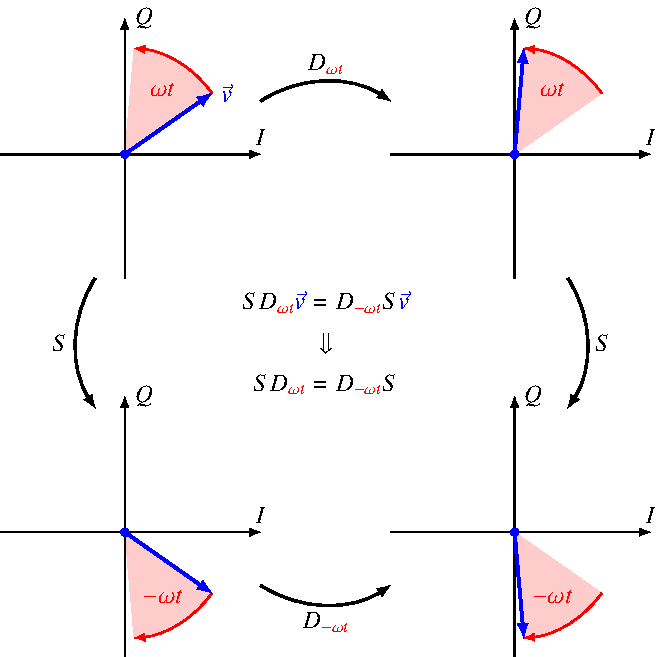
\includegraphics{applications/qam/images/spiegelung.pdf}
\caption{Vertauschungsregel für die Drehmatrizen $D_{\pm\omega t}$ und
die Matrix $S$ der Spiegelung an der $I$-Achse.
\label{figure:qam:spiegelung}}
\end{figure}
Zusammen bewirken sie dasselbe wie eine Drehung um $\omega t$ gefolgt
von einer Spiegelung an der $I$-Achse, also
\[
D_{-\omega t}S=SD_{\omega t}.
\]
Damit erhalten wir
\[
D_{-\omega t}PD_{\omega t}
=
\frac12E + \frac12 SD_{2\omega t},
\]
woraus wieder die Formel~\eqref{eqn:qam:filter}
für $\hat{v}(t)$ folgt.

\subsubsection{Filterung des Trägers}
\begin{figure}
\centering
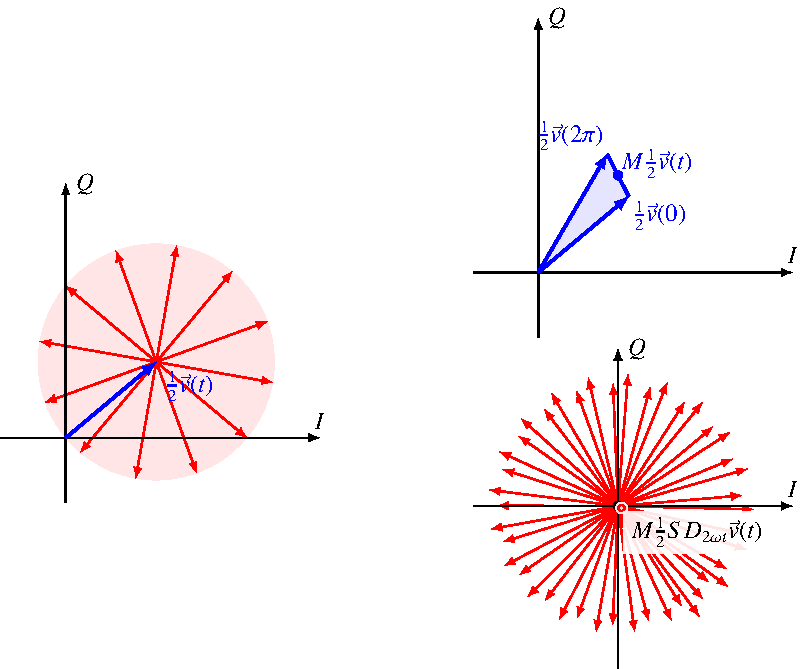
\includegraphics{applications/qam/images/filter.pdf}
\caption{Filterung des Trägers aus~\eqref{eqn:qam:filter}
links für ein konstantes Signal $\vec{v}(t)=\vec{v}(0)$, rechts
für ein langsam veränderliches Signal.
Zur besseren Lesbarkeit sind rechts die Terme
$\frac12\vec{v}(t)$ oben und $\frac12SD_{2\omega t}\vec{v}(t)$
unten getrennt.
Der Mittelwerte $\mathcal{M}\frac12SD_{2\omega t}$ ist der Beitrag des
zweiten Terms zum Mittelwert und sehr nahe beim Nullpunkt,
die Mittelung über ein Periodenintervall des Trägers bringt die
Trägerkomponente also fast vollständig zum Verschwinden.
\label{figure:qam:filter}}
\end{figure}
Gehen wir davon aus, dass die Bewegung des Vektors $\vec{v}(t)$ in
der $I$-$Q$-Ebene sehr viel langsamer ist als die Drehung mit der
Winkelgeschwindigkeit $2\omega$, dann können wir den zweiten Term
näherungsweise eliminieren.
Um dies zu verstehen, nehmen wir an, dass $\vec{v}(t)$ während eines
Zeitintervalls der Länge $L=\pi/\omega$ konstant ist ist.
Wir bezeichnen Mittelwerte über das Intervall mit dem Buchstaben $\mathcal{M}$.
Wir beachten dann, dass der zweite Term in \eqref{eqn:qam:filter}
für dieses Zeitintervall die gleichförmige, ganze Drehung des Vektors
um den Nullpunkt beschreibt.
Der Mittelwert des zweiten Terms über das Intervall verschwindet daher:
\[
\mathcal{M}\frac12SD_{2\omega t}\vec{v}(t)
=
0
\]
(siehe auch Abbildung~\ref{figure:qam:filter} links).
Der erste Term von \eqref{eqn:qam:filter} ist während des Intervalls
konstant, ihr Mittelwert ist daher
\[
\mathcal{M}\frac12\vec{v}(t)
=
\frac12\vec{v}(t).
\]
Wir finden daher den Mittelwert
\[
\mathcal{M}\hat{v}(t)
=
\frac12\vec{v}(t),
\]
bis auf den Faktor $\frac12$ wird also $\vec{v}(t)$ durch die Mittelwertbildung
rekonstruiert.
Verändert sich $\vec{v}(t)$ während des Intervalls um einen Betrag
kleiner als $\varepsilon$ (Abbildung~\ref{figure:qam:filter} rechts),
dann kommt ein Fehler hinzu, der ebenfalls
von der Grössenordnung $\varepsilon$ ist.

In praktischen Anwendungen ist die Frequenz des Trägers mehrere
Grössenordnungen grösser als die typischen Frequenzen in $I(t)$ 
und $Q(t)$, die Annahme, dass sich $\vec{v}(t)$ während einer halben
Trägerperiode nicht ändert, ist daher mit grosser Genauigkeit erfüllt.
Die Mittelwertbildung wird technisch mit Hilfe eines Tiefpassfilters
realisiert.

\subsubsection{Demodulationsfehler}
Bis jetzt sind wir davon ausgegangen, dass wir die Frequenz und die
Phase des Trägersignals genau kennen.
Doch dies ist nicht korrekt.
Die Demodulation erfolgt im Empfänger, wo die Matrix $D_{\omega t}$
neu erzeugt werden muss.
Dabei kann es zu Fehlern in der Frequenz kommen.
Die Demodulation erfolgt also mit einer Matrix $D_{\omega_rt}$
mit einer möglicherweise von der Sendefrequenz $\omega$
abweichenden Frequenz $\omega_r=\omega+\Delta\omega$.
Das decodierte Signal ist dann
\begin{equation}
\begin{aligned}
\hat{v}(t)
&=
D_{-\omega_rt}PD_{\omega t}\vec{v}(t)
=
D_{-(\omega+\Delta\omega)t} ({\textstyle\frac12}E+{\textstyle\frac12}S)
D_{\omega t}\vec{v}(t)
=
\frac12D_{-\Delta\omega t}\vec{v}(t)
+
\frac12D_{-(\omega+\Delta\omega)t}SD_{\omega t}\vec{v}(t)
\\
&=
\frac12 D_{-\Delta\omega t}\vec{v}(t)
+
\frac12 SD_{(\omega +\Delta\omega) t}D_{\omega t}\vec{v}(t)
=
\frac12 D_{-\Delta\omega t}\vec{v}(t)
+
\frac12 SD_{(2\omega +\Delta\omega) t}\vec{v}(t)
\end{aligned}
\label{eqn:qam:demoomegar}
\end{equation}
Bei der Filterung des Trägers verschwindet der zweite Term.
Die Demodulation liefert also nicht den Vektor $\vec{v}(t)$, vielmehr
rotiert der demodulierte Vektor mit der Winkelgeschwindigkeit $\Delta\omega$.

Korrekte Demodulation ist also nur möglich, wenn Sender und Empfänger exakt
die gleiche Frequenz verwenden.
Der Empfänger kann versuchen, die korrekte Frequenz aus dem empfangenen
Signal zu extrahieren, oder Sender und Empfänger können ein hochgenaues
Frequenznormal verwenden.
Ein Rubidium-Frequenznormal stellt eine Referenz-Frequenz mit einem
typischen relativen Fehler kleiner als $10^{-9}$ zur Verfügung.
Bei einem Trägersignal im typischen Bereich der Mobiltelefonie (Grössenordnung
$\sim 1\,\text{GHz}$) resultiert also weniger als eine Umdrehung von $\hat{v}(t)$
pro Sekunde.

Selbst wenn Sender und Empfänger hochgenaue Frequenzreferenzen verwenden,
wenn man also annehmen darf, dass $\omega_r=\omega$,
ist noch nicht sichergestellt, dass auch die Phase übereinstimmt.
Die Demodulation könnte mit einer um den Winkel $\delta$
phasenverschobenen Drehmatrix $D_{\omega t+\delta}$ erfolgen.
Die selbe Rechnung wie in \eqref{eqn:qam:demoomegar} liefert dann
\[
\hat{v}(t)
=
\frac12D_{-\delta}\vec{v}(t)
+
\frac12SD_{\delta+2\omega t}\vec{v}(t).
\]
Bei der Filterung fällt auch hier der zweite Term weg, der demodulierte
Vektor ist aber um den Winkel $-\delta$ verdreht.
Um dies zu vermeiden muss der Sender dem Empfänger die genaue Phase
irgendwie mitteilen.
Technische Möglichkeiten dazu werden in den nachstehenden Beispielen
kurz angesprochen.







